\chapter{Evaluation}

\section{\bb 3 alignment benchmark dataset}
\begin{wrapfigure}{r}{0.4\textwidth}
	\centering
	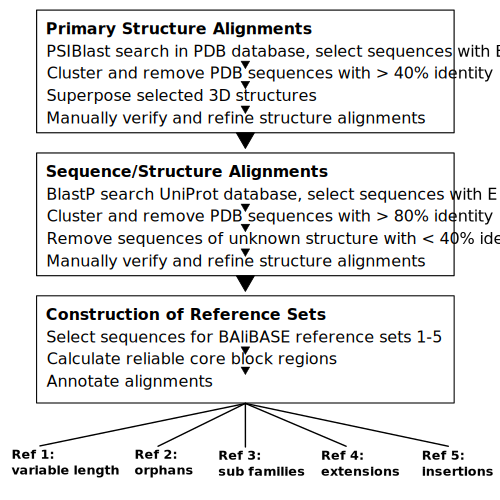
\includegraphics[width=0.5\textwidth]{./images/balibase.png}
	\caption{Semi automatic process used to establish the reference sets. Source: \cite{hundt2020praktkium}}
	\label{fig:balibase}
\end{wrapfigure}

The third version of the \bb benchmark protein alignment database has been released in 2005 and is widely employed for the comparison of multiple alignment programs \cite{thompson2005balibase, Russell2016}. It is constructed in a semi automatic process as shown in \cref{fig:balibase} and suitable to evaluate global and local alignment programs. The database is split into 5 reference sets with different characteristics representing distinctive multiple alignment problems. \\
It is divided into:



\begin{itemize}
	\item reference set 1 subset V1, for which any two sequences share <20\% identity and no internal insertions over 35 residues long
	\item reference set 1 subset V2, consisting of families with at least four equidistant sequences for which any two sequences share 20-40\% identity and no large insertions
	\item reference set 2, for which all sequences share >40\% identity and at least one 3D structure is known. Additionally an "Orphan" sequence with <20\% identity is chosen per family
	\item for reference set 3, all sequences in the same subfamily have >40\% identity, whereas sequences from different subfamilies share <20\% identity
	\item for reference sets 4 and 5, every sequence shares at least 20\% with one other sequence, including sequences with large N/C-terminal extensions (ref 4) or internal insertions (ref 5)
\end{itemize}

\subsection{Core blocks}

Evaluating and comparing alignment programs is a difficult problem due to the uncertainty of supposedly "real" alignments of actual sequences. The \bb database  marks alignment columns which can be reliably aligned as so called "core blocks". These core blocks are calculated and manually verified, making up 19\% of the full length sequences which are used in the evaluation of \textit{spam-align} \cite{thompson2005balibase}.

%\begin{itemize}
%	\item what are core blocks?
%	\item how are they determined and validated?
%\end{itemize}

\begin{figure}[h]
	\centering
	\includegraphics[width=0.8\textwidth]{./images/balibase-web.png}
	\caption{\bb web interface. Black columns indicate core blocks. \href{www.lbgi.fr/wscoperr?Balibase&FileMoi&macsimHtml&BB20006}{lbgi.fr}}
	\label{}
\end{figure}

\subsection{Quality of Alignments}

Quality measures for protein alignment benchmarks \\
https://academic.oup.com/nar/article/38/7/2145/3100529


\section{Sum-of-pairs and column score}
Comparing the alignment output of different methods can be done by computing the sum-of-pairs and column scores.\\
Given a test alignment $A_t$ and a reference alignment $A_r$ with $M$ sequences and $N_t, N_r$ columns respectively, the sum-of-pairs and column score is defined according to Thompson et al. \cite{thompson1999comprehensive}.

\begin{mydef}[Sum-of-pairs score]
	The sum of pairs score is the ratio of correctly aligned individual residues. Formally it is defined as:
	\begin{align*}
		p_{ijk} &= \begin{cases}
		1 \text{ if residues $A_{t{_ij}}$ and $A_{t_{ik}}$ \textbf{are} aligned in $A_r$}\\
		0 \text{ otherwise}
		\end{cases} \\
		S_i &= \sum_{j=1}^{M} \sum_{k=i+1}^{M} p_{ijk} \\
		SPS &= \frac{\sum_{i=1}^{N_t} S_i} {\sum_{i=1}^{N_r} S_{r_i}}
 	\end{align*}
 	with $S_{r_i}$ being the number of correctly aligned residues in the reference.
\end{mydef}

\begin{mydef}[Column score]
	The column score is the ratio of correctly aligned columns. 
	\begin{align*}
	C_i &= \begin{cases}
	1 \text{ if all the residues in the i-th column are aligned correctly}\\
	0 \text{ otherwise}
	\end{cases} \\
	CS &= \frac{\sum_{i=1}^{N_t} C_i}{N_r}
	\end{align*}
\end{mydef}
Note that $C_i = 1$ only if all the residues in the $i$-th column are aligned correctly and no residue belonging to this column is part of another one. For this reason, the numerator is smaller or equal to the denominator.\\
The definition of the column score is slightly different than that provided by the authors of \bb \cite{thompson1999comprehensive} but resembles the actual implementation in the included BaliScore tool and its reimplementation provided with this thesis.\\
These scores are only calculated for the core blocks of the \bb alignments, meaning that for the following evaluation $A_t$ is an alignment over the full sequences, while $A_r$ contains only the aligned residues inside the core blocks.


\section{Bali-Score}
Accompanying this thesis is a reimplementation of the \textit{bali-score} tool, which can be used to calculate the SPS and column scores given a test alignment in \code{fasta} format and a \bb reference \code{xml} file. Although some of the features part of the original implementation or not part of this version, it is not dependent on the \textit{Expat XML parser}, which proved to be burdensome.\\
The source code is available on \href{TODO github url}{github.com} and, provided the current stable Rust toolchain \footnote{View \href{https://rustup.rs}{rustup.rs} for installation instruction} is available, installing the tool can simply be done by issuing \code{cargo install --path .} in the cloned repository root. For usage instructions view \code{bali-score -h}.



\section{Evaluated programs}


\subsection{Mafft}
Mafft (version 7), standing for \textbf{m}ultiple \textbf{a}lignment using \textbf{f}ast \textbf{F}ourier \textbf{t}ransform, is a widely used similarity based multiple sequence alignment program employing progressive, iterative and structural strategies \cite{katoh2013mafft}.



\begin{itemize}
	\item mafft offers plethora of strategies for different situations
	\item two strategies are evaluated
	\begin{itemize}
		\item here referred to as Mafft-Fast: FFT-NS-1 (very fast; recommended for >2000 sequences; progressive method with a rough guide tree): mafft --retree 1 --maxiterate 0 input [> output]
		\item here referred to as Mafft-Accurate: L-INS-i (probably most accurate; recommended for <200 sequences; iterative refinement method incorporating local pairwise alignment information): mafft --localpair --maxiterate 1000 input [> output]
	\end{itemize}
\end{itemize}

\textit{MAFFT} is evaluated for two different alignment strategies, from now on referred to as \textit{fast} and \textit{accurate}

\subsection{Dialign}

\subsection{Spam-Align}


\begin{itemize}
	\item which pattern sets have been used? -> include rasbhari parameters
\end{itemize}


\section{Results}

\begin{itemize}
	\item execution times include finding of micro alignments which is unnecessarily complex atm. and takes up roughly 50\% of program run time 
\end{itemize}

\begin{figure}[h]
	\centering
	\includegraphics[width=0.8\textwidth]{../alignment-evaluation/sop-by-pattern-params.png}
	\caption{Sum of pairs scores aggregated over \bb reference sets and weights.}
	\label{}
\end{figure}
\begin{figure}[H]
	\centering
	\includegraphics[width=0.8\textwidth]{../alignment-evaluation/cs-by-pattern-params.png}
	\caption{Column scores aggregated over \bb reference sets and weights.}
	\label{}
\end{figure}

Table shows sum-of-pairs scores for compared programs (only selected parameters for spam-align).
3
\begin{tabular}{lrrrrrr}
\toprule
{} &      RV11 &      RV12 &      RV20 &      RV30 &      RV40 &      RV50 \\
\midrule
Dialign             &  0.494482 &  0.851870 &  0.868279 &  0.739987 &  0.830939 &  0.804629 \\
Mafft-Accurate      &  0.648562 &  0.937168 &  0.927191 &  0.862048 &  0.917403 &  0.899301 \\
Mafft-Fast          &  0.521931 &  0.890052 &  0.885096 &  0.812195 &  0.842169 &  0.850608 \\
spam-align-w-2\_d-11 &  0.238148 &  0.718407 &  0.847409 &  0.713624 &  0.782116 &  0.726905 \\
spam-align-w-3\_d-10 &  0.222217 &  0.688189 &  0.840199 &  0.712141 &  0.778949 &  0.716480 \\
\bottomrule
\end{tabular}


\begin{figure}[h]
	\centering
	\includegraphics[width=0.8\textwidth]{../alignment-evaluation/sop-boxplot.png}
	\caption{Sum of pairs scores. Spam-Align is called with a pattern of weight 2 and 11 don't care positions.}
	\label{}
\end{figure}
\begin{figure}[h]
	\centering
	\includegraphics[width=0.8\textwidth]{../alignment-evaluation/cs-boxplot.png}
	\caption{Column scores. Spam-Align is called with a pattern of weight 2 and 11 don't care positions.}
	\label{}
\end{figure}

\begin{figure}[h]
	\centering
	\includegraphics[width=0.8\textwidth]{../alignment-evaluation/time-by-pattern-params.png}
	\caption{Mean execution times in ms.}
	\label{}
\end{figure}
